%!TEX root = prelim.tex
%!TEX root = fakeroot.tex


% Alignment
\subsection{Sparse Representation with Warping}
\frame{\frametitle{Compound Effect of Alignment and Illumination}
\renewcommand{\imagesizestring}{height}
\renewcommand{\imagesizea}{0.25\textheight}
\renewcommand{\imagesizeb}{0.15\textheight}
\renewcommand{\gapsizea}{-0mm}
\begin{tabular}[b]{cc@{}b{.5\textwidth}}
% Example for setting the heights of the images
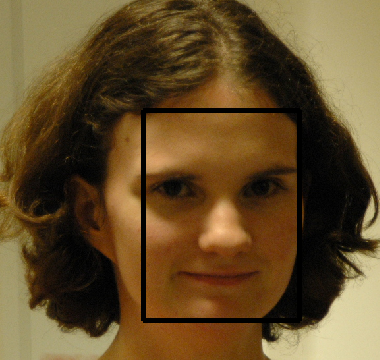
\includegraphics[\imagesizestring=\imagesizea]{figures_cvpr/promo/case1/detector.png}& \hspace{\gapsizea}
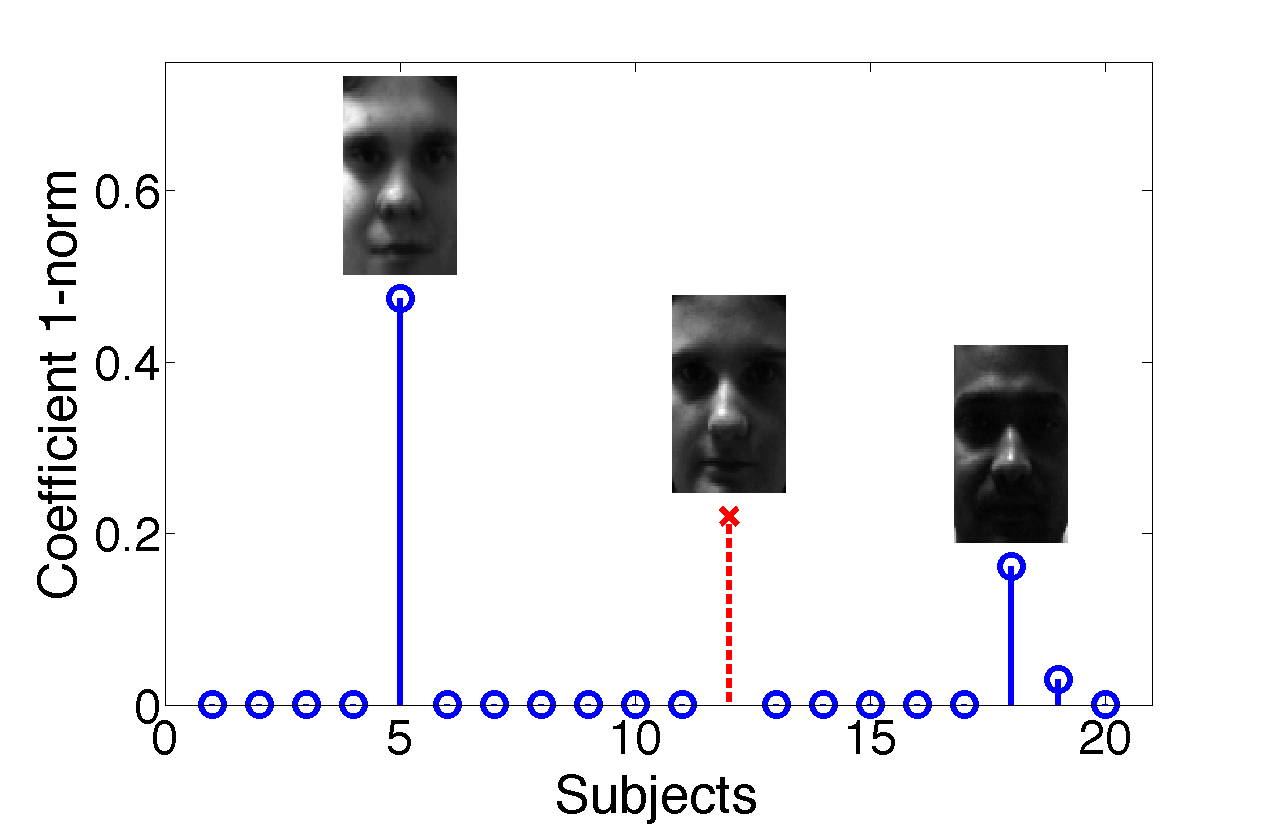
\includegraphics[\imagesizestring=\imagesizea]{figures_cvpr/promo/case1/sci_with_axis_face_case1.png} & 
{\bf Poor alignment}, Sufficient training illuminations \vfill\\
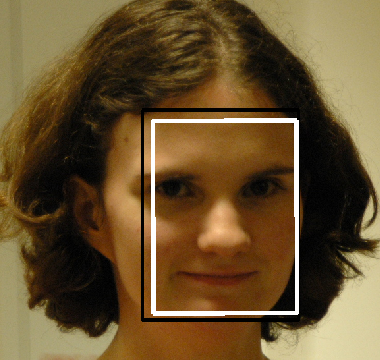
\includegraphics[\imagesizestring=\imagesizea]{figures_cvpr/promo/alignment_and_detector.png}& \hspace{\gapsizea}
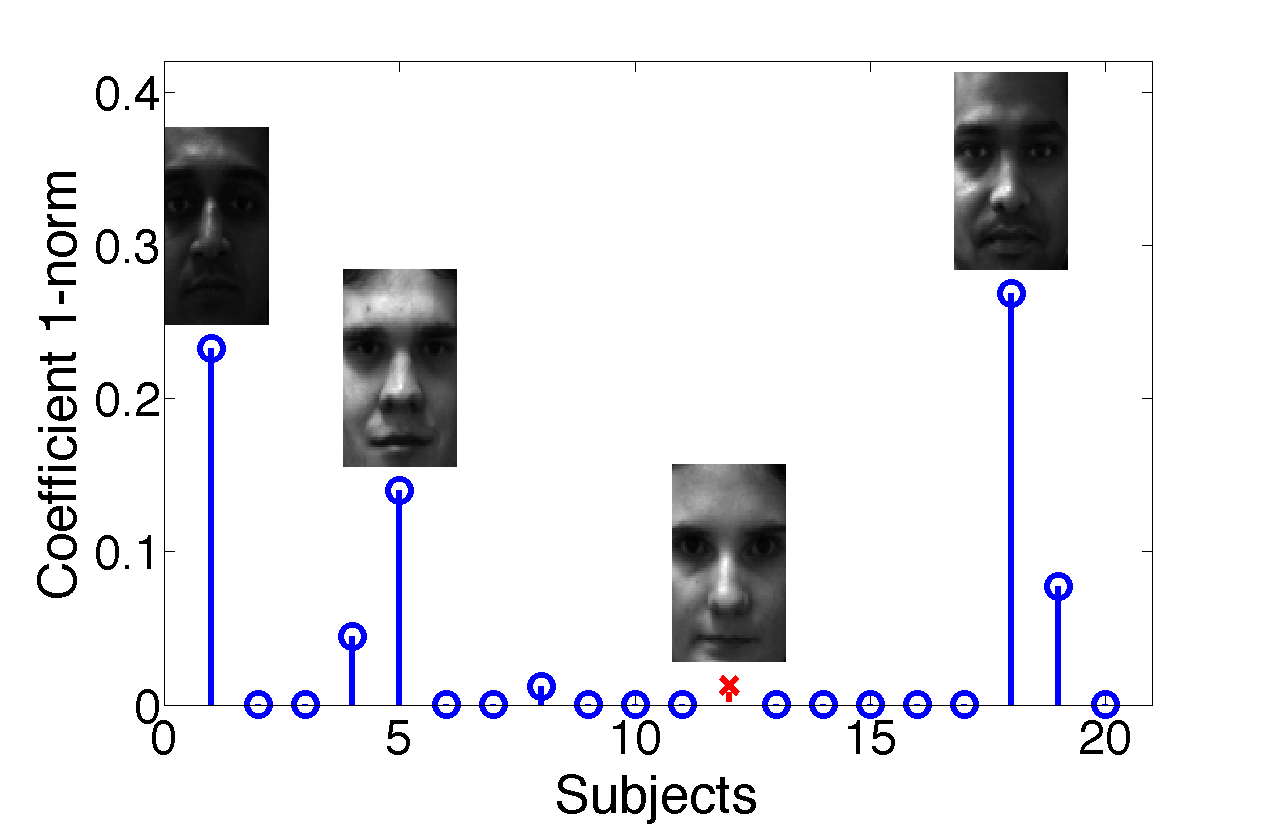
\includegraphics[\imagesizestring=\imagesizea]{figures_cvpr/promo/case2/sci_with_axis_face_case2.png} & 
{{\bf Good alignment}, Insufficient training illuminations}\vfill\\
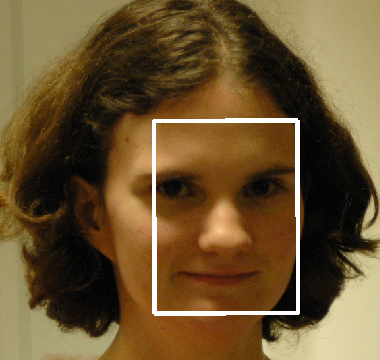
\includegraphics[\imagesizestring=\imagesizea]{figures_cvpr/promo/case3/alignment.png} & \hspace{\gapsizea}
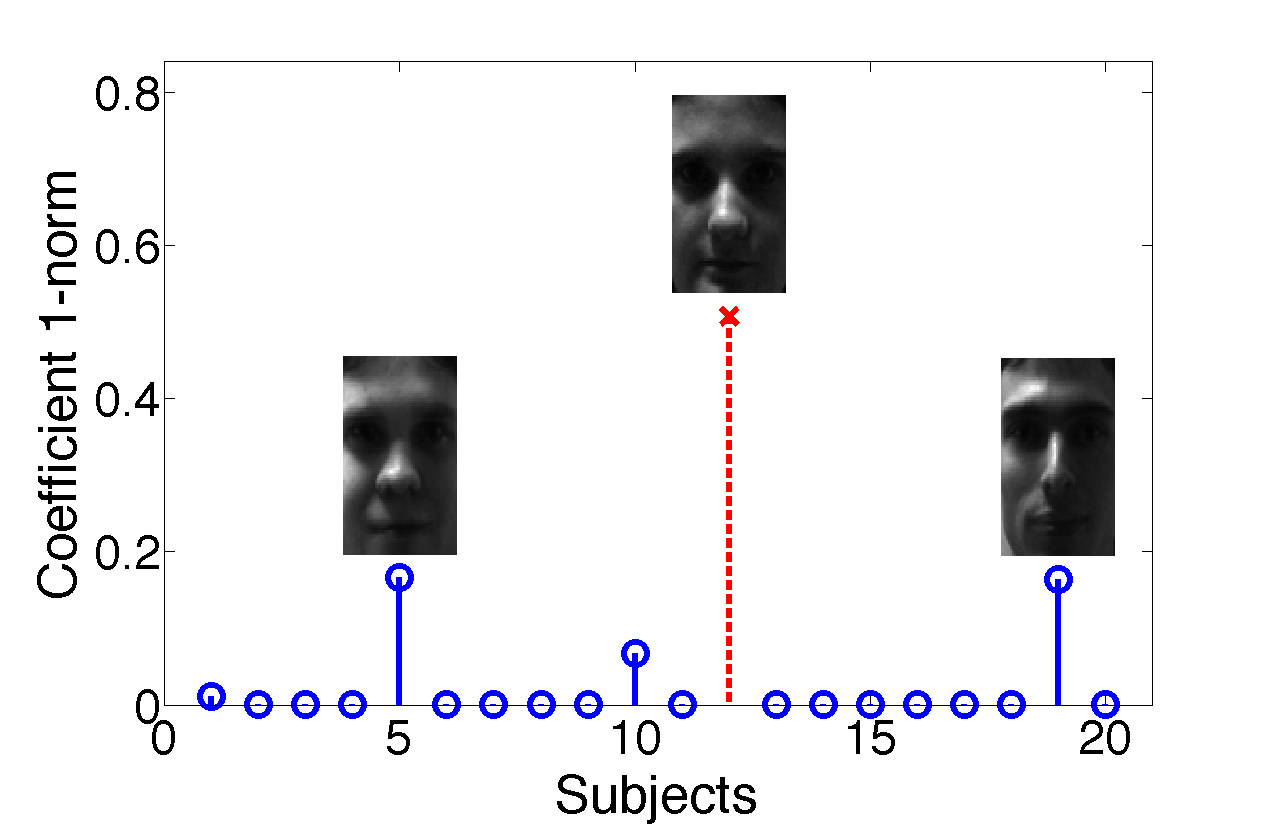
\includegraphics[\imagesizestring=\imagesizea]{figures_cvpr/promo/case3/sci_with_axis_face_case3.png} &
{{\bf Good alignment}, Sufficient training illuminations}\vfill
\end{tabular}
}

\frame{
\frametitle{Image Embedding}
\vspace{-3mm}
\begin{center}
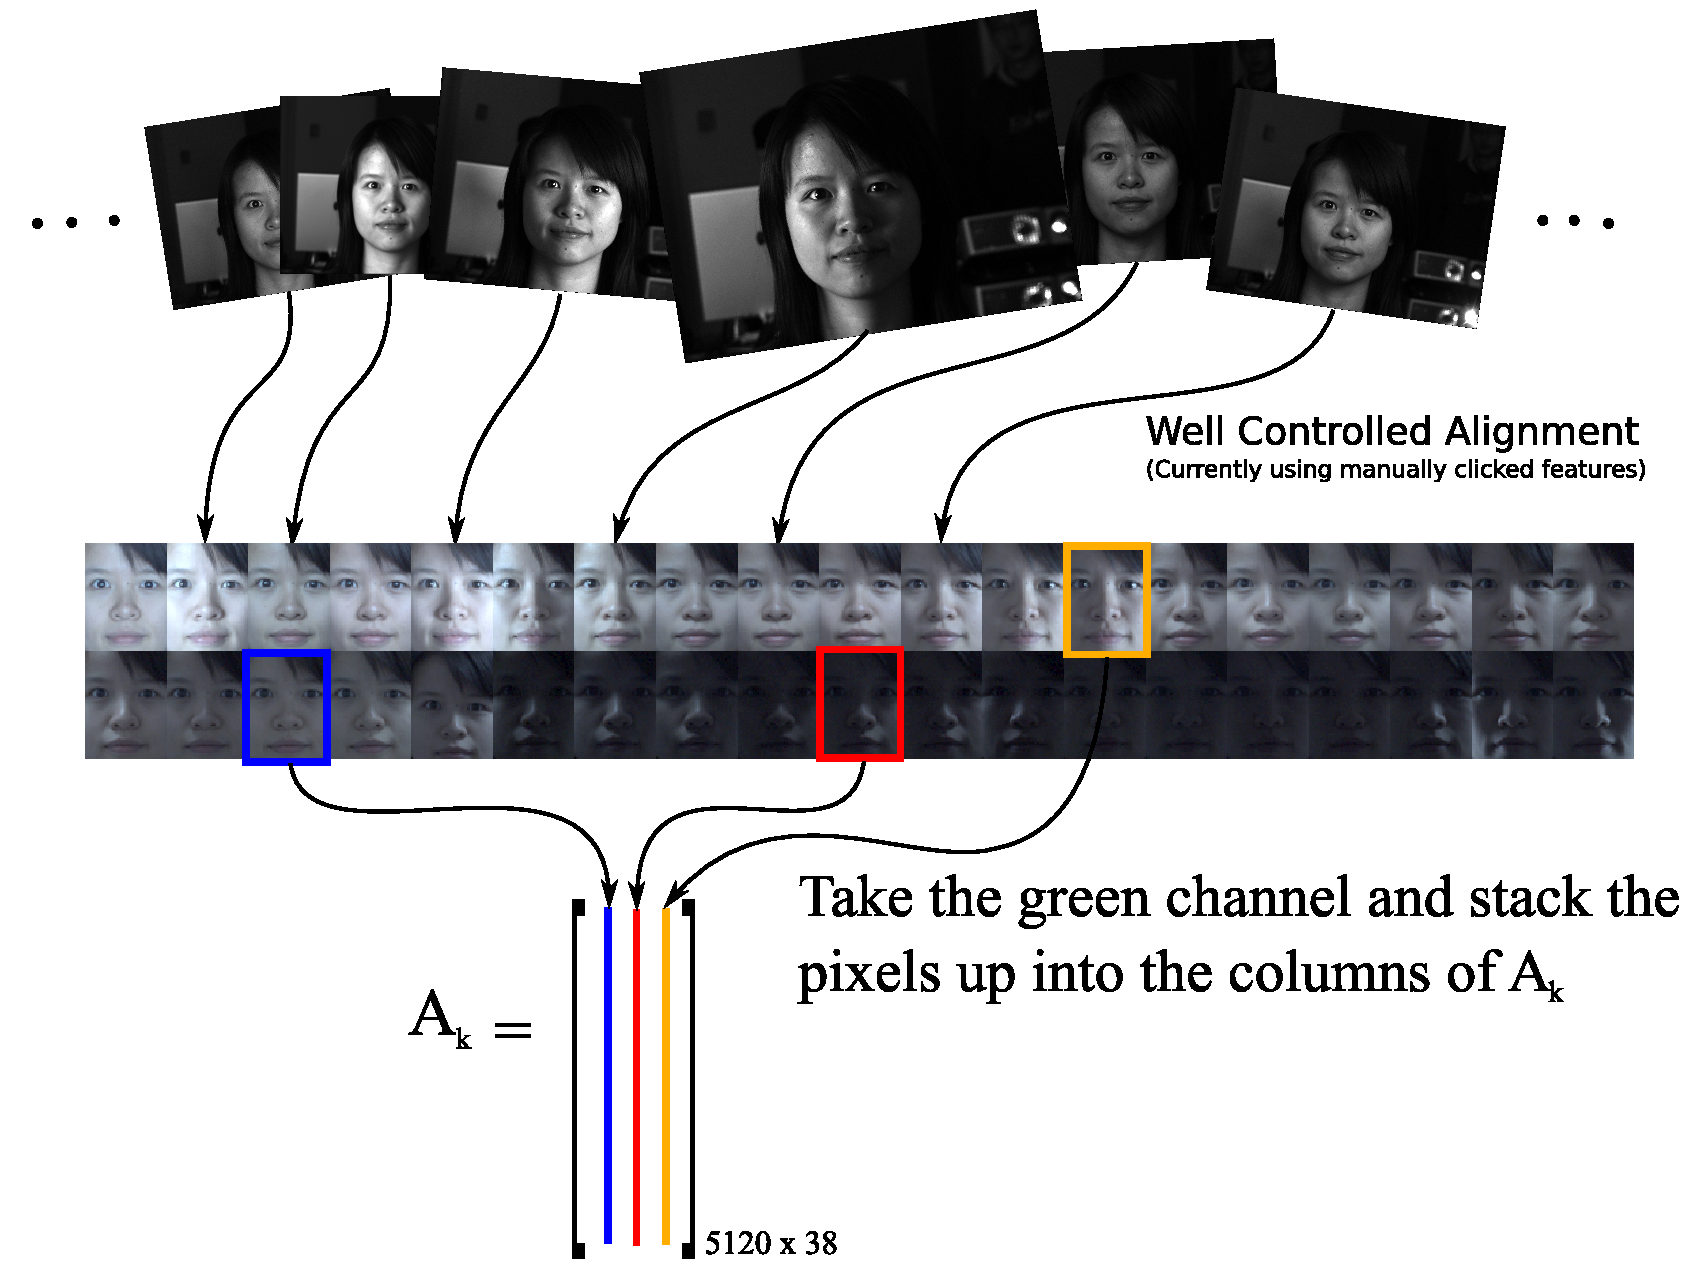
\includegraphics[width=.70\textwidth]{figures_embedding/training_embedding.pdf}\\
$A = [ A_1 \mid A_2 \mid \dots \mid A_K ] \in \Re^{m \times n}$
\end{center}
}

\frame{
\frametitle{Sparse Representation with Warping}
\vspace{-.1in} {\footnotesize
\begin{itemize}
\item<1-> SRC uses the following minimization:
\begin{equation*}
(\hat{\x}, \hat{\e}) = \argmin{\x,\e} \| \x \|_1 + \| \e\|_1 \quad \subj \quad \underbrace{\y_0}_{\mbox{\tiny test image}} = \underbrace{A}_{\mbox{\tiny training data}} \underbrace{\x}_{\mbox{\tiny coefficients}} + \underbrace{\e}_{\mbox{\tiny sparse error}}
\end{equation*}
\begin{center}{\color{blue} Assumes $\y$ aligned}\end{center}
\item<2-> For an un-aligned test image:
\begin{equation*}
(\hat{\x}, \hat{\e}, \hat{\tau}) = \argmin{\x,\e,\tau \in T} \| \x \|_1 + \| \e \|_1 \quad \subj \quad  \underbrace{\y}_{\mbox{\tiny un-aligned}} \circ \underbrace{\tau}_{\mbox{\tiny transformation}} = A \x + \e
\end{equation*}
\begin{center}{\color{blue}many local minima! scales badly!}\vspace{-.05in}\end{center}
\item<3-> Per-User alignment:
\begin{equation*}
(\hat \x, \hat \e,\hat \tau_i) = \argmin{\x,\e,\tau_i \in T} \| \e \|_1 \quad \subj \quad \y \circ \tau_i = A_i \x + \e
\end{equation*}
\begin{center}{\color{blue}not convex!}\vspace{-.05in}\end{center}
\item<4-> Linearize w.r.t. parameterization of $\tau$:
\begin{equation*}
(\hat \x, \hat \e, \Delta\hat\tau_i) = \argmin{\x,\e,\Delta\tau_i \in T} \| \e \|_1 \quad \subj \quad \y\circ \tau + \underbrace{J}_{\mbox{\tiny Jacobian}} \Delta \tau_i = A_i \x + \e
\end{equation*}
\end{itemize}
}}

\frame{
\frametitle{Iterative Alignment}
\begin{itemize}
\item Since we linearized $\y \circ \tau_i$, we have to iterate between solving
\begin{eqnarray*}
(\hat \x, \hat \e, \Delta\hat\tau_i) &\leftarrow& \argmin{\x,\e,\Delta\tau_i \in T} \| \e \|_1 \quad \subj \quad \y\circ \tau_i + J \Delta \tau_i = A_i \x + \e \\
\tau_i &\leftarrow& \tau_i + \Delta\hat \tau_i
\end{eqnarray*}
and re-computing the Jacobian $J$ about the new point $\y\circ (\tau_i + \Delta \tau_i)$.
\item To avoid degenerate solutions, normalize the {\em warped} test image:
\begin{equation*}
\tilde\y(\tau) = \frac{\y\circ\tau}{||\y\circ\tau||_2}
\end{equation*}
\item Normalize columns of $A$ to unit $\ell^2$ norm.
\item Enforce constraint $\x>0$.
\item Can extend this to multiscale
\end{itemize}
}

\frame{
\frametitle{Recognition Step}
\begin{itemize}
\item Re-sample training database using inverted $\tau_i$ from alignment step:
\begin{equation*}
A \leftarrow \left[ A_1 \circ \tau_1^-1 \ldots A_i \circ \tau_i^-1\ldots \right]
\end{equation*}
\item Perform global optimization:
\begin{equation*}
(\hat{\x}, \hat{\e}) = \argmin{\x,\e} \| \x \|_1 + \| \e\|_1 \quad \subj \quad \y = \underbrace{A}_{\mbox{\tiny aligned}} \x + \e
\end{equation*}
\item Return user with lowest residual $||\y - A_i \hat x_i||_2$. 
\end{itemize}
}

\frame{
\frametitle{Recognition Pipeline}
\begin{center}
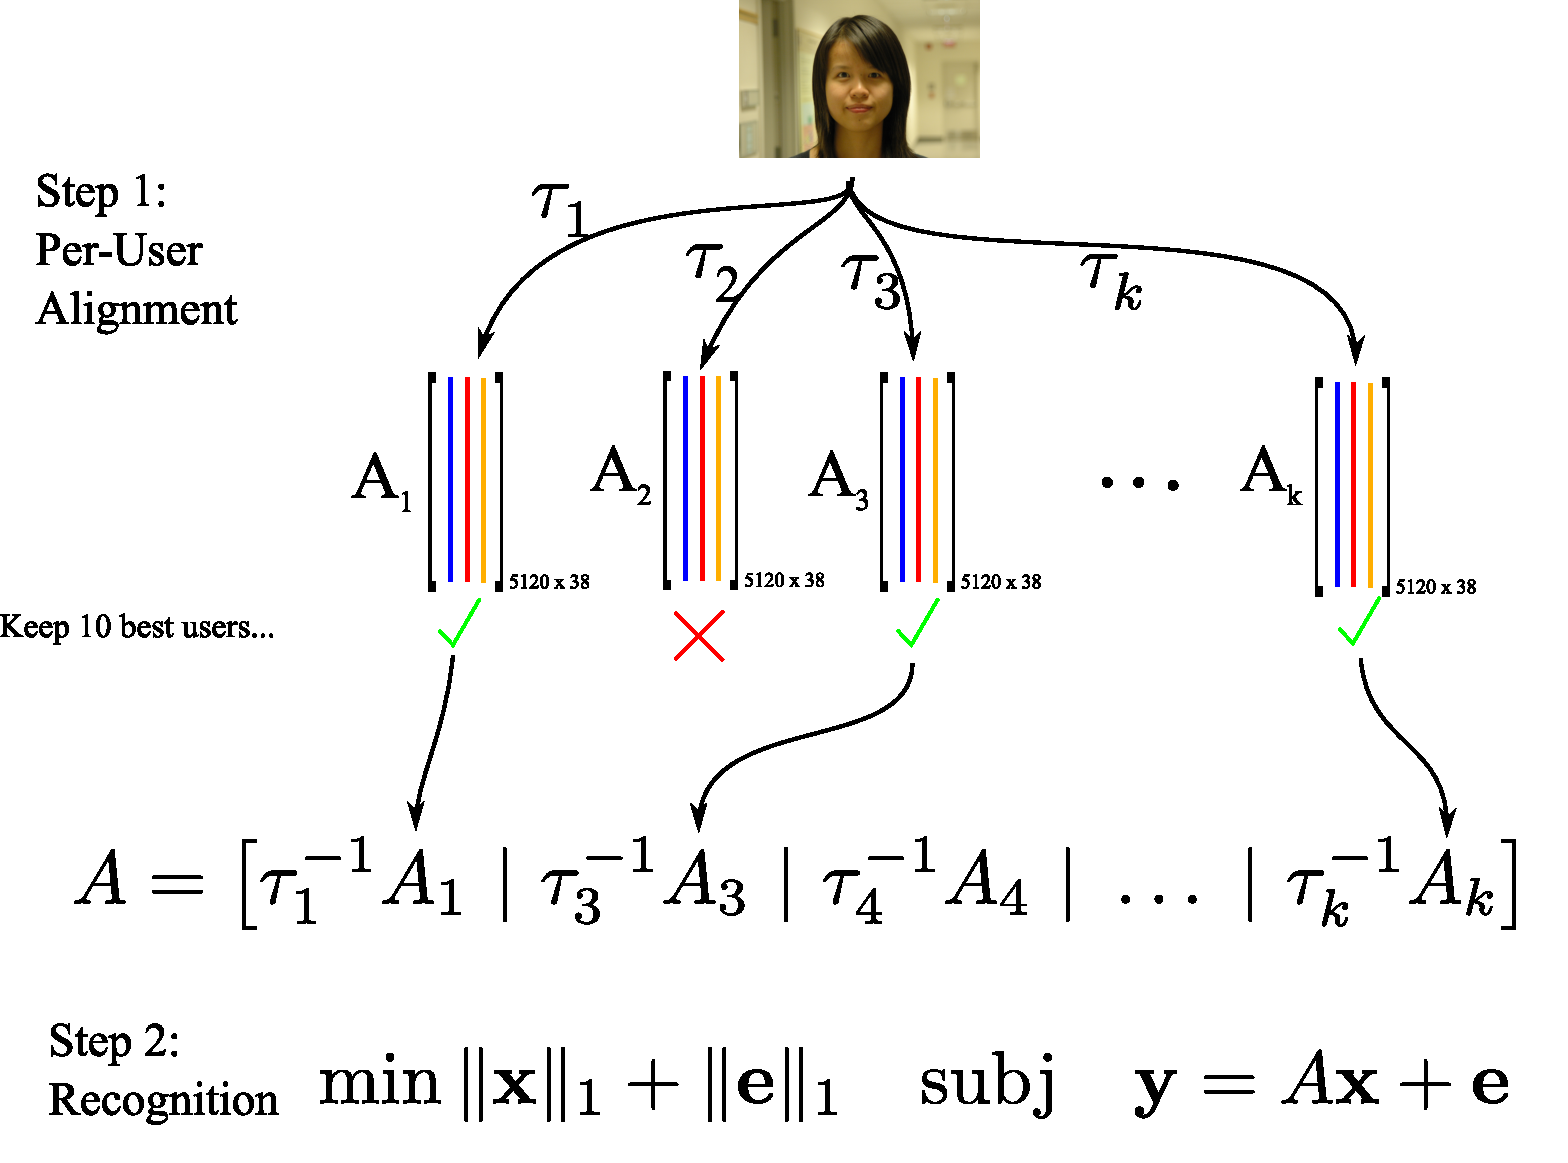
\includegraphics[width=.75\textwidth]{figures_embedding/pipeline.pdf}
\end{center}
}


%\frame{\frametitle{Alignment Examples}
%$\ell^1$ and $\ell^2$ minimization alignment comparison
%\begin{columns}
%\begin{column}{0.5\textwidth}
%\renewcommand{\imagesizestring}{height}
%\renewcommand{\imagesizea}{0.2\textheight}
%\begin{tabular}[t]{@{}c@{}c@{}c@{}c@{}m{.2\textwidth}}
%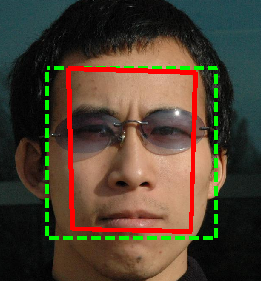
\includegraphics[\imagesizestring=\imagesizea]{figures_cvpr/L1_cropped} &
%
\includegraphics[\imagesizestring=\imagesizea]{figures_cvpr/y_warp_L1} &
%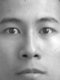
\includegraphics[\imagesizestring=\imagesizea]{figures_cvpr/y_hat_L1} &
%
\includegraphics[\imagesizestring=\imagesizea]{figures_cvpr/e_L1} &
%$\|\e\|_1$\\[-.05in]
%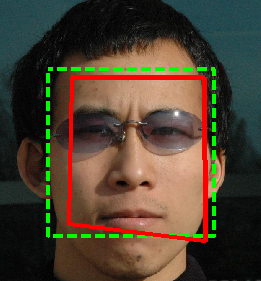
\includegraphics[\imagesizestring=\imagesizea]{figures_cvpr/L2_cropped} &
%
\includegraphics[\imagesizestring=\imagesizea]{figures_cvpr/y_warp_L2} &
%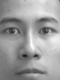
\includegraphics[\imagesizestring=\imagesizea]{figures_cvpr/y_hat_L2} &
%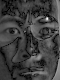
\includegraphics[\imagesizestring=\imagesizea]{figures_cvpr/e_L2} &
%$\|\e\|_2$ \\[-.1in]
%{\tiny Face Boundary} & {\tiny Aligned Test} & {\tiny Reconstruction} & {\tiny $|$Error$|$}
%\end{tabular}
%\end{column}
%\begin{column}{0.5\textwidth}
%\renewcommand{\imagesizestring}{height}
%\renewcommand{\imagesizea}{0.2\textheight}
%Alignment tolerance for out-of-plane pose variation
%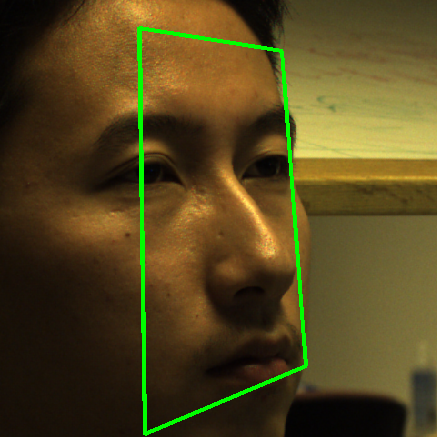
\includegraphics[\imagesizestring=\imagesizea]{figures_cvpr/21}
%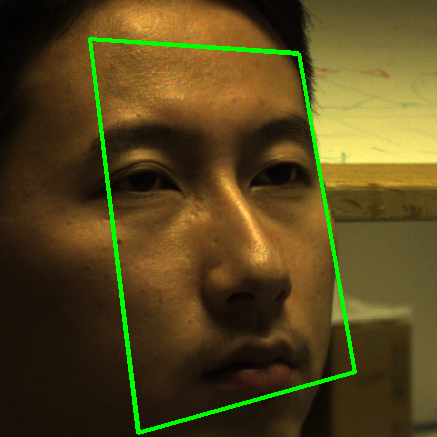
\includegraphics[\imagesizestring=\imagesizea]{figures_cvpr/19}
%
\includegraphics[\imagesizestring=\imagesizea]{figures_cvpr/17}
%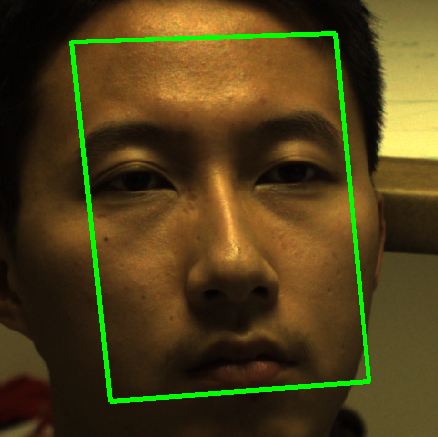
\includegraphics[\imagesizestring=\imagesizea]{figures_cvpr/15}
%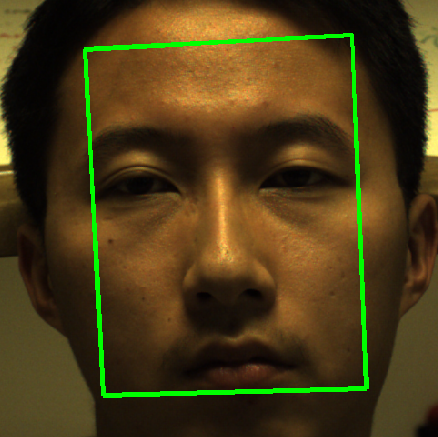
\includegraphics[\imagesizestring=\imagesizea]{figures_cvpr/13}\\
%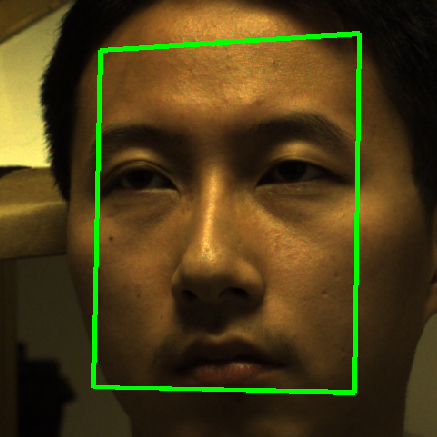
\includegraphics[\imagesizestring=\imagesizea]{figures_cvpr/11}
%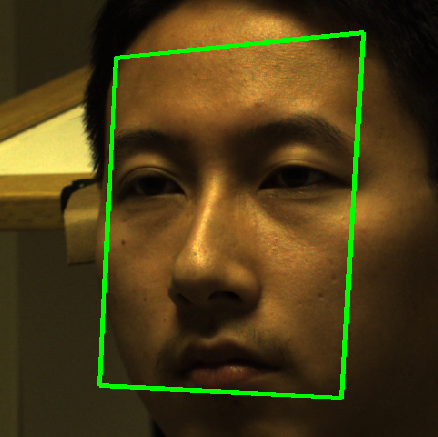
\includegraphics[\imagesizestring=\imagesizea]{figures_cvpr/09}
%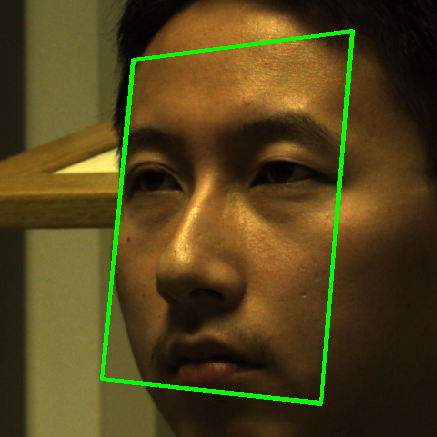
\includegraphics[\imagesizestring=\imagesizea]{figures_cvpr/7}
%
\includegraphics[\imagesizestring=\imagesizea]{figures_cvpr/5}
%
\includegraphics[\imagesizestring=\imagesizea]{figures_cvpr/3}\\
%Alignment using a projective transformation works up to about $45^{\circ}$.
%\end{column}
%\end{columns}
%}

\subsection{Experiments}




\renewcommand{\imagesizestring}{height}
\renewcommand{\imagesizea}{0.36\textheight}
\renewcommand{\gapsizea}{-0mm}
\frame{\frametitle{Alignment region of attraction}
%\begin{tabular}{cc}
\begin{center}
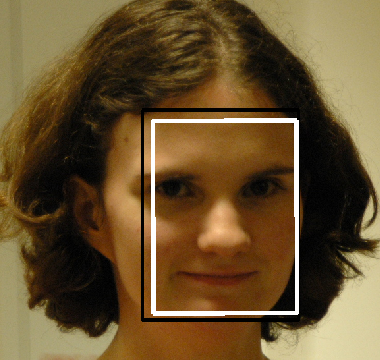
\includegraphics[\imagesizestring=\imagesizea]{figures_cvpr/promo/alignment_and_detector.png}
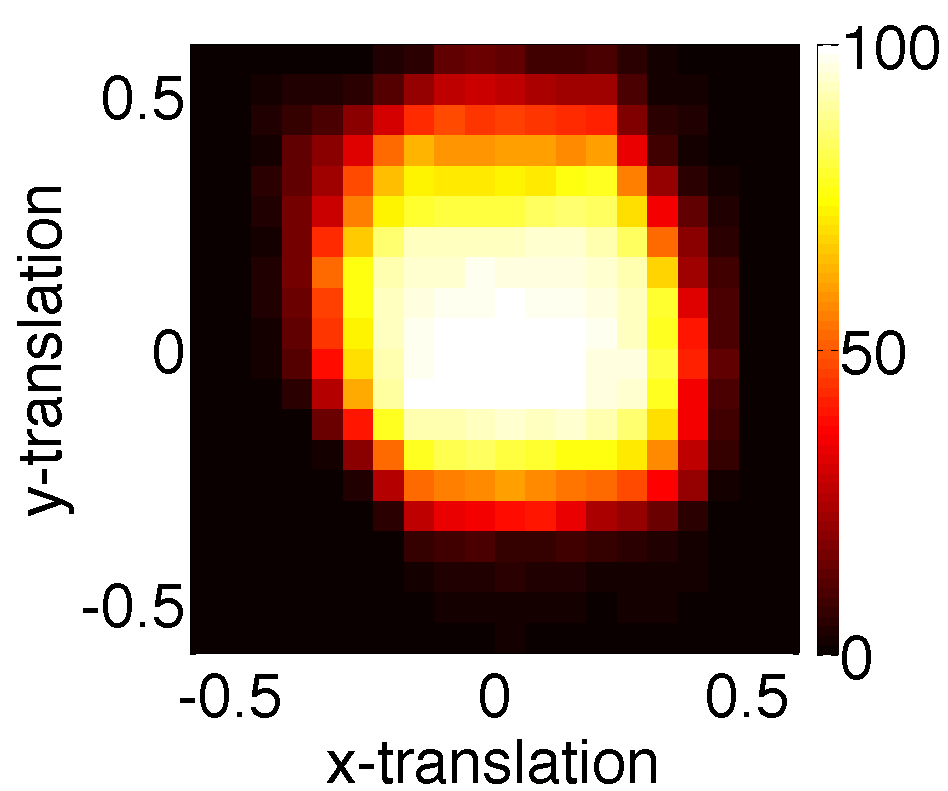
\includegraphics[\imagesizestring= \imagesizea]{figures_cvpr/translation_fig3.png}
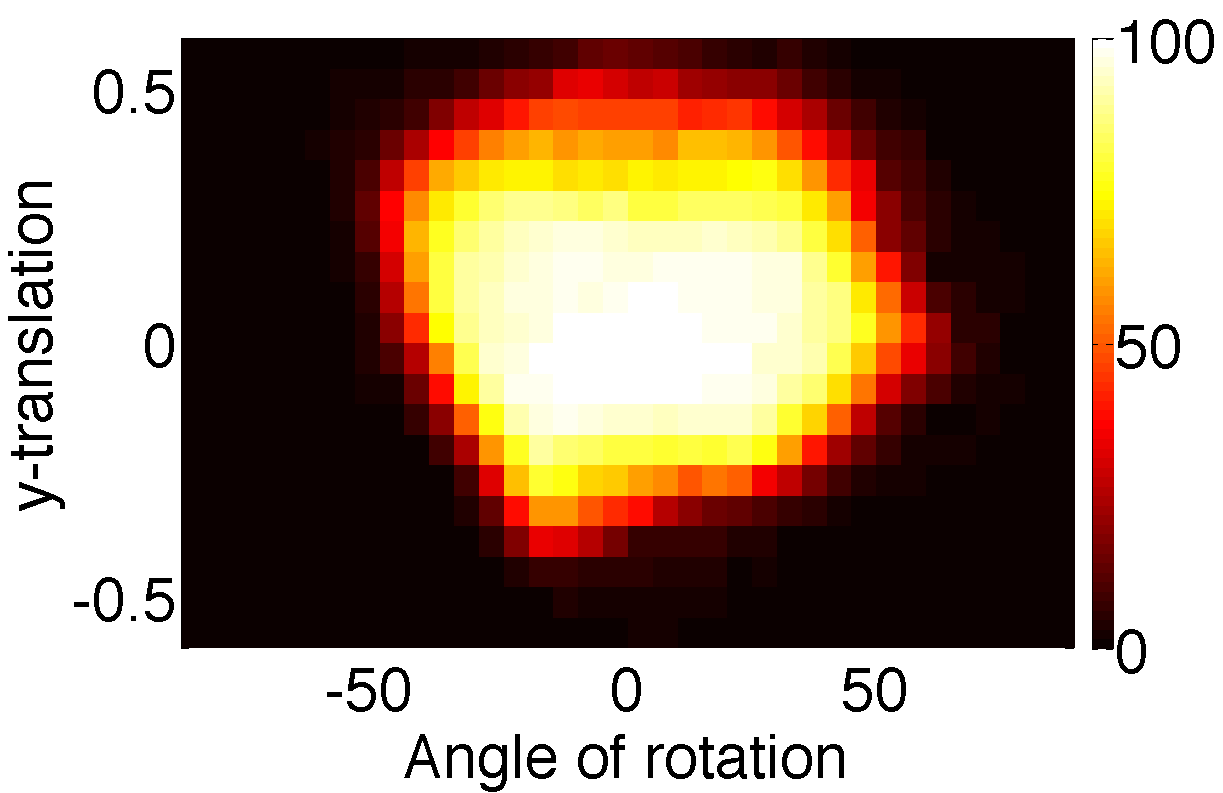
\includegraphics[\imagesizestring= \imagesizea]{figures_cvpr/translation_rotation_fig1.png}
\end{center}
%\end{tabular}
\vspace{0mm}
{\tiny
\begin{itemize}
\item Translation is expressed as a fraction of outer eye corner distance.
\item In-plane rotation is expressed in degrees. 
\item Probability of convergence from synthetic transformations to hand-clicked ground truth
\item Training: CMU Multi-PIE, 120 subjects, 11 illuminations, session 2.  Re-sampled to $60 \times 80$ pixels.
\item Testing: 1 new illumination from session 3
\item Viola Jones' face detector average error on this data set falls safely within our region of attraction
\end{itemize}}
}


\frame{\frametitle{Alignment Examples}
{\footnotesize
\vspace{-.1in}
Comparison of $\ell^1$ and $\ell^2$ minimization:
\renewcommand{\imagesizestring}{height}
\renewcommand{\imagesizea}{0.15\textheight}
\vspace{-.05in}
\begin{center}
\begin{tabular}[t]{b{.3in}cccc}
$\min \|\e\|_2$\vfill &
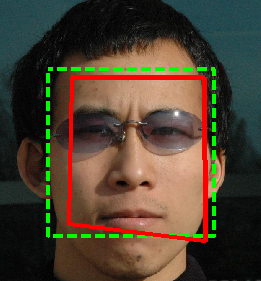
\includegraphics[\imagesizestring=\imagesizea]{figures_cvpr/L2_cropped} &

\includegraphics[\imagesizestring=\imagesizea]{figures_cvpr/y_warp_L2} &
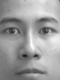
\includegraphics[\imagesizestring=\imagesizea]{figures_cvpr/y_hat_L2} &
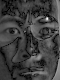
\includegraphics[\imagesizestring=\imagesizea]{figures_cvpr/e_L2} \\
$\min \|\e\|_1$\vfill &
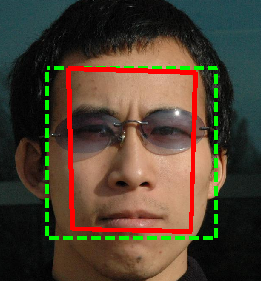
\includegraphics[\imagesizestring=\imagesizea]{figures_cvpr/L1_cropped} &

\includegraphics[\imagesizestring=\imagesizea]{figures_cvpr/y_warp_L1} &
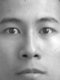
\includegraphics[\imagesizestring=\imagesizea]{figures_cvpr/y_hat_L1} &

\includegraphics[\imagesizestring=\imagesizea]{figures_cvpr/e_L1} \\
& {\tiny Face Boundary} & {\tiny Aligned Test} & {\tiny Reconstruction} & {\tiny $|$Error$|$}
\end{tabular}
\end{center}

%$\ell^1$ and $\ell^2$ minimization alignment comparison
\renewcommand{\imagesizestring}{height}
\renewcommand{\imagesizea}{0.15\textheight}
\vspace{-.1in}

%Alignment tolerance for out-of-plane pose variation
Alignment using a projective transformation works up to about $45^{\circ}$.
\vspace{-.05in}
\begin{center}
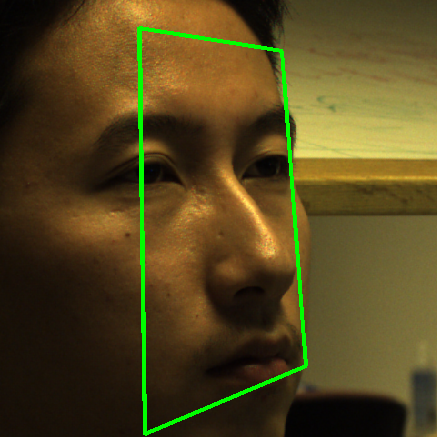
\includegraphics[\imagesizestring=\imagesizea]{figures_cvpr/21}
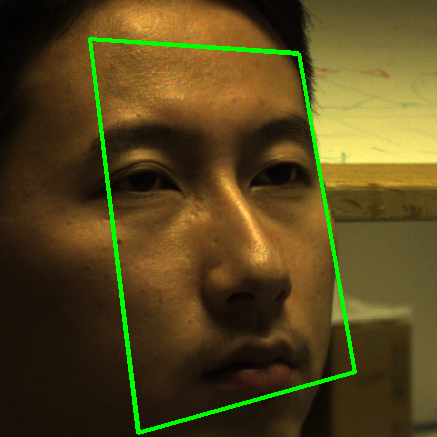
\includegraphics[\imagesizestring=\imagesizea]{figures_cvpr/19}

\includegraphics[\imagesizestring=\imagesizea]{figures_cvpr/17}
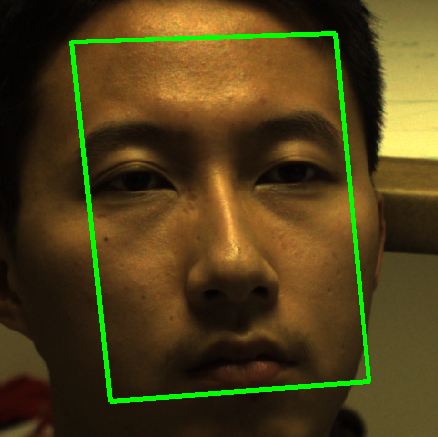
\includegraphics[\imagesizestring=\imagesizea]{figures_cvpr/15}
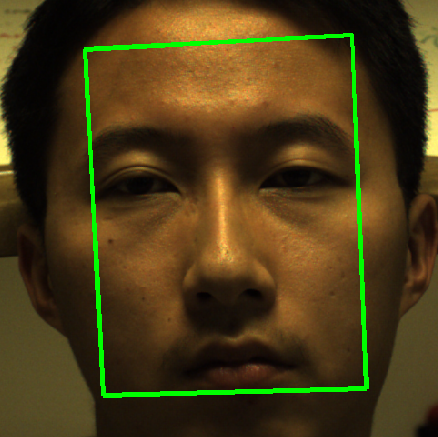
\includegraphics[\imagesizestring=\imagesizea]{figures_cvpr/13}\\
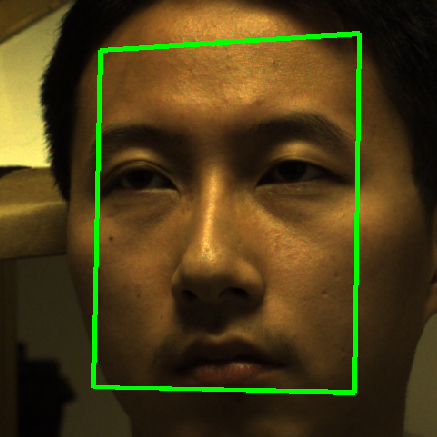
\includegraphics[\imagesizestring=\imagesizea]{figures_cvpr/11}
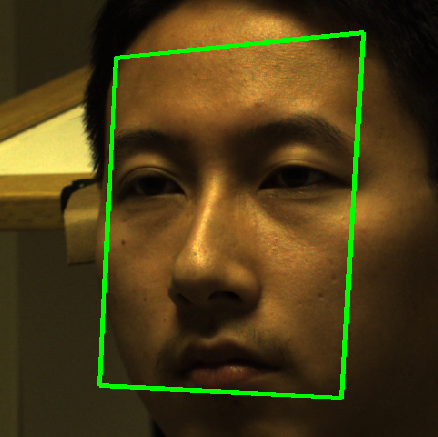
\includegraphics[\imagesizestring=\imagesizea]{figures_cvpr/09}
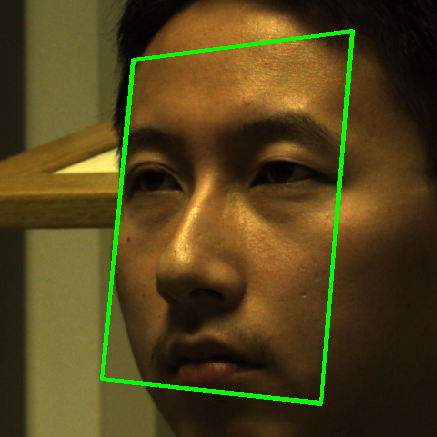
\includegraphics[\imagesizestring=\imagesizea]{figures_cvpr/7}

\includegraphics[\imagesizestring=\imagesizea]{figures_cvpr/5}

\includegraphics[\imagesizestring=\imagesizea]{figures_cvpr/3}\\
\end{center}}
}
